\documentclass[11pt,a4paper]{article}
\usepackage[T1]{fontenc}
\usepackage[utf8]{inputenc}
\usepackage{lmodern}
\usepackage[margin=23mm]{geometry}
\usepackage{graphicx}
\usepackage{float}
\usepackage{amsmath}
\usepackage{booktabs,tabularx}
\usepackage{enumitem}
\usepackage{xcolor}
\usepackage{listings}
\usepackage{microtype}
\usepackage{fancyhdr}
\usepackage[hidelinks]{hyperref}
\graphicspath{{figures/}}
\setlength{\parindent}{0pt}
\setlength{\parskip}{6pt}
\setlength{\emergencystretch}{2em}
\setlist{itemsep=3pt,topsep=4pt}
\lstset{basicstyle=\ttfamily\footnotesize,breaklines=true,columns=fullflexible,keepspaces=true,frame=single,rulecolor=\color{black!25},backgroundcolor=\color{black!3}}
\pagestyle{fancy}
\fancyhf{}
\fancyhead[L]{\small RasPi MilliTome Software Manual}
\fancyhead[R]{\small 17 November 2026}
\fancyfoot[C]{\thepage}
\setlength{\headheight}{14pt}
\newcommand{\button}[1]{\textbf{#1}}
\newcommand{\manualfigure}[4]{\begin{figure}[H]\centering\includegraphics[width=#2\linewidth,height=#3\textheight,keepaspectratio]{#1}\caption{#4}\end{figure}}
\title{The RasPi MilliTome Software\\\large Acquisition and Reconstruction Manual}
\author{Danilo Roccatano}
\date{Updated 17 November 2026}
\begin{document}
\maketitle
\section{Overview and quick start}
This manual covers image acquisition with Raspberry Pi Camera Module~3 and reconstruction of serial-section image stacks on a separate computer. It also identifies the retained acquisition script for the earlier Camera V1.3 configuration. The original photographs are preserved throughout the workflow.

\begin{enumerate}
\item Prepare the specimen and camera, select an output folder, focus on the slicing surface and keep the imaging geometry fixed.
\item Photograph each exposed surface in sequence, recording the physical advancement between photographs.
\item Open the image folder in the reconstruction program. Existing \path{segmentation_params.json} settings are loaded automatically when valid.
\item For a new dataset, select the calibrated ROI, enter its physical width and the recorded slice spacing, and inspect HSV segmentation across representative slices.
\item Press \button{Accept ALL} to generate masks, sectional areas and a volume estimate.
\item Use \button{3D View} and, after creating the mesh, \button{Export STL} for visualization or fabrication.
\end{enumerate}

\textbf{Equipment.} Acquisition requires a Raspberry Pi with a compatible camera and camera software, illumination, and a monitor, keyboard and mouse. A dedicated TFT is not required for the current interface. Reconstruction requires a computer with Python, Tk, NumPy, OpenCV, Pillow, SciPy, scikit-image and PyVista/VTK. These are the dependencies used by the supplied scripts; install camera-specific dependencies on the Raspberry Pi and reconstruction dependencies on the analysis computer.

\textbf{Screenshots.} Images in this manual show the author's actual acquisition and reconstruction interfaces. Values visible during a demonstration are not universal defaults. For reproducible quantitative processing, use the complete saved settings belonging to the selected dataset.

\clearpage
\section{Camera Module 3 acquisition interface}
The Camera Module~3 program uses Picamera2. Figure~\ref{fig:acquisition} shows the live preview, focus controls, capture button and saved-file status. The displayed sensor dimensions and configured capture dimensions are different quantities; saved image size alone does not identify the camera model.
\begin{figure}[H]
\centering
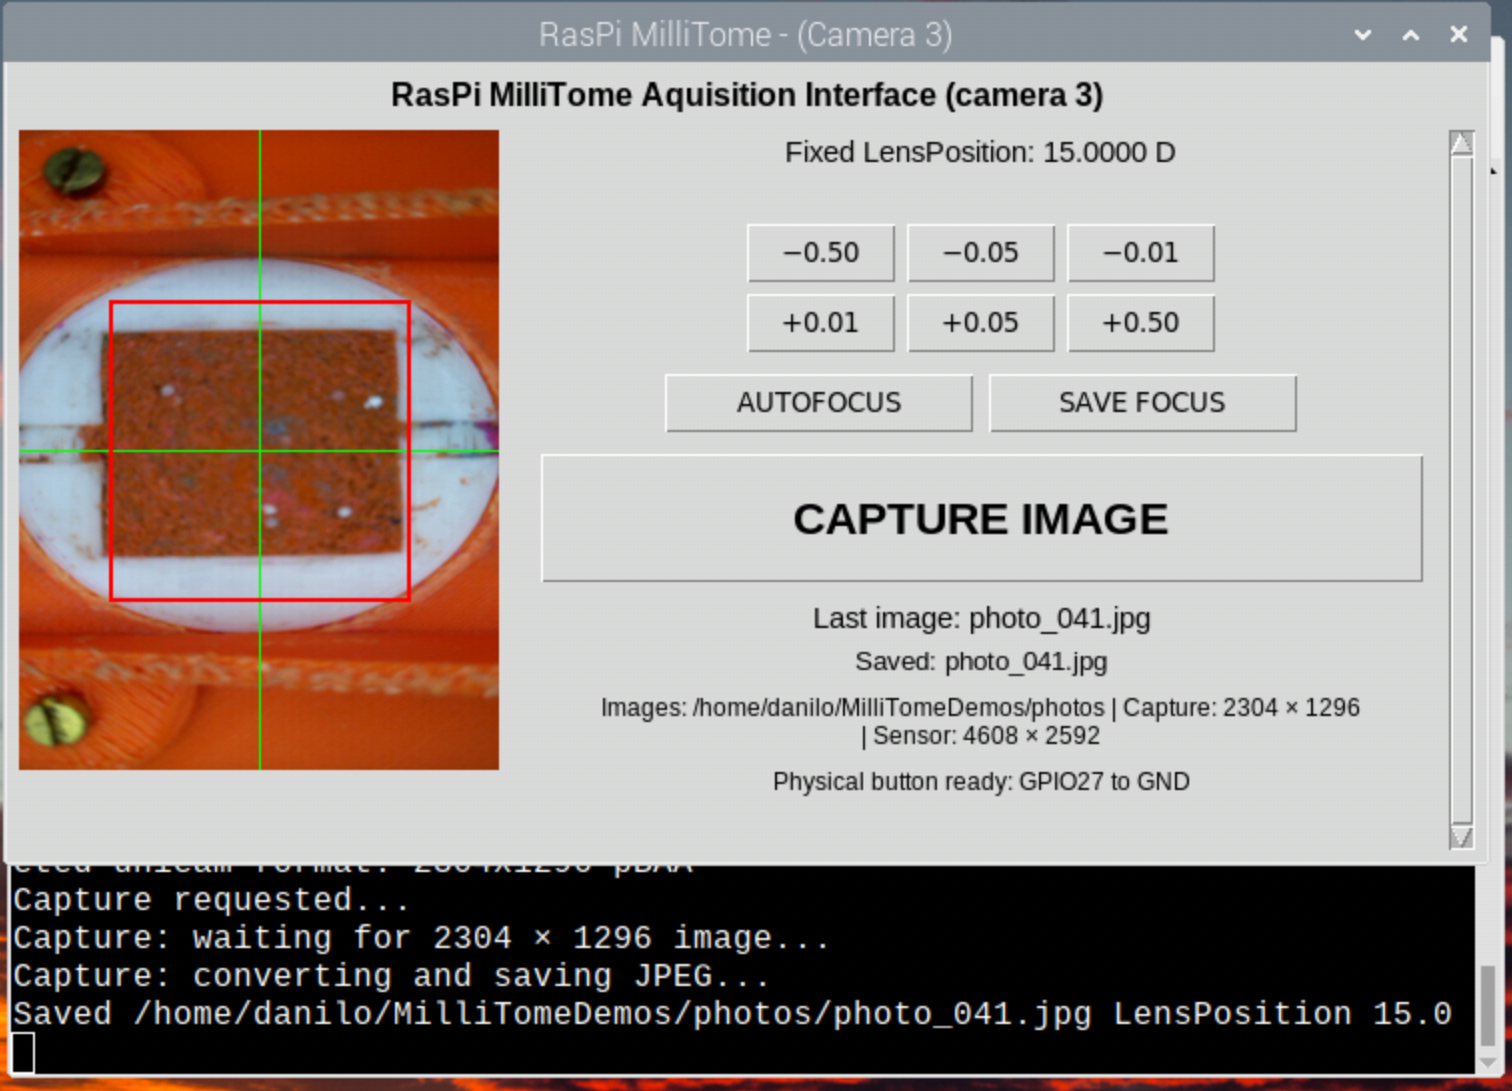
\includegraphics[width=\linewidth]{acquisition_camera3.png}
\caption{Camera Module~3 acquisition interface. The preview includes alignment guides. The status identifies the most recently saved photograph, output directory and capture dimensions. A short terminal confirmation is also visible below the application.}
\label{fig:acquisition}
\end{figure}
\begin{itemize}
\item \button{AUTOFOCUS}: focus on the specimen surface, then hold the resulting lens position for subsequent captures.
\item \button{$-0.50$, $-0.05$, $-0.01$ / $+0.01$, $+0.05$, $+0.50$}: make coarse or fine manual adjustments to the displayed lens position.
\item \button{SAVE FOCUS}: save the current lens position for later use. Recheck focus when camera height or the specimen plane changes.
\item \button{CAPTURE IMAGE}: request and save the next photograph. Wait for the saved-file confirmation before advancing or cutting again.
\end{itemize}
The red box and crosshairs assist alignment; they do not establish the physical ROI calibration used for reconstruction.

\clearpage
\section{Acquisition procedure and camera versions}
\subsection{Starting and recording a sequence}
The repository's compact Camera Module~3 acquisition script is:
\begin{quote}\path{Acquisition/RasPiMilliTome_Picamera2_Focus_v2_GPIO27_Zero2W_Compact.py}\end{quote}
Run it with Python on the Raspberry Pi. From the repository root:
\begin{lstlisting}
python3 Acquisition/RasPiMilliTome_Picamera2_Focus_v2_GPIO27_Zero2W_Compact.py
\end{lstlisting}
A locally renamed copy may have a different filename, as in the screenshot; use the filename actually supplied with the repository.

\begin{enumerate}
\item Mount the camera securely above the cutting plane and arrange steady illumination. Connect the external display and input devices.
\item Check the output folder before starting a new specimen. The compact script uses \path{~/MilliTomeDemos/photos}; use an empty folder or archive the previous sequence to avoid combining specimens.
\item Adjust focus at the exposed specimen surface, then keep the camera geometry and lens position fixed through the sequence.
\item Capture a surface, wait for the saved-file confirmation, advance by the recorded interval, cut, and capture the next exposed surface. Keep this convention consistent and record any missing sections or interventions.
\item Retain the full sequence, including blank end sections, together with the acquisition log.
\end{enumerate}
The script numbers files as \path{photo_001.jpg}, \path{photo_002.jpg}, and so on, continuing after the highest existing number. The focus file is \path{~/MilliTomeDemos/millitome_camera_focus.json}. Camera settings, when supplied, are read from \path{~/MilliTomeDemos/camera_settings.json}.

The optional physical capture switch connects GPIO27 to ground (BCM numbering; header pin~13). The GUI capture button is also available. Follow the wiring for the selected script; a physical switch is not required to operate the software through the GUI.

\subsection{Legacy Camera V1.3 support}
\path{Acquisition/RasPiMilliTome_Acquisition.py} is the retained Camera V1.3 program. It imports the legacy \texttt{picamera} library and requires a compatible legacy camera software stack. Its TFT and GPIO interface differs from the Camera Module~3 program. Use the script and dependencies appropriate to the camera configuration; the legacy script is not the Camera Module~3 acquisition program.

\clearpage
\section{Loading an image stack for reconstruction}
Start the reconstruction program on the analysis computer:
\begin{lstlisting}
python3 Reconstruction/RasPiMilliTome_Reconstruction.py
\end{lstlisting}
If your distributed copy has a suffix such as \texttt{\_FIXED}, substitute that filename. A photo folder may also be supplied as a command-line argument.

Press \button{Load} and select the folder containing one specimen's original photographs. The application displays the current image, its segmentation mask and the coloured overlay. Use \button{Prev} and \button{Next} to inspect the sequence.
\manualfigure{reconstruction_loaded.png}{1}{0.43}{Current reconstruction interface after loading a magenta-background image stack. The empty mask can be appropriate for an initial section containing only background sand.}

\subsection{Automatic settings loading}
When the selected folder contains a valid \path{segmentation_params.json}, the application restores its ROI, original image dimensions, source-image order, HSV thresholds, physical width, axial spacing, morphology and blob-filter settings. The displayed controls are synchronized with those values.

\button{Load Params} restores another saved JSON file, subject to validation. It is not a way to reuse one dataset's geometry for another: source filenames, image sizes and the physical ROI must belong to the selected stack. Mismatches or invalid settings must be resolved before processing.

The message \textbf{``reprocess required''} means that no valid current batch volume is available. Press \button{Accept ALL} after the settings have been checked.

\clearpage
\section{Selecting and calibrating the ROI}
For a new dataset, press \button{ROI} and select the opening or reference region whose physical dimensions are known. Confirm the selection in the ROI window. The current quantitative implementation requires a square image ROI.
\manualfigure{roi_selection.png}{0.48}{0.53}{Selecting the specimen region in the original photograph. Use the visible physical opening or independently calibrated reference boundaries, rather than the green inclusion boundary.}

\textbf{ROI physical width (mm)} is the actual width represented by the selected pixels. If an ROI has width $n$ pixels and represents $L$~mm, the scale is $s=L/n$~mm per pixel. The green region's sectional area is its foreground pixel count multiplied by $s^2$.

Changing ROI width while leaving $L$ unchanged changes the calculated scale, even if the green foreground pixels do not change. Choose the ROI from the physical boundaries, independently of the desired volume. A marked rim can improve selection consistency.

For an existing example, restore its saved JSON and do not select the ROI again unless deliberately revising its calibration. Each dataset needs its own ROI and image metadata. A rectangular physical calibration would require separate horizontal and vertical scales; it is not implemented by the current square-ROI tool.

\clearpage
\section{HSV segmentation and morphological cleanup}
Press \button{HSV Tune} to display the minimum and maximum hue, saturation and value controls. Inspect an early, central and late inclusion section, as well as background-only sections. A suitable mask should include the intended material while limiting unwanted background selection.
\manualfigure{hsv_preview.png}{1}{0.43}{Preview while adjusting HSV thresholds. This demonstration shows a temporary value minimum of 41 and an invalidated volume; the common example settings below use 40.}

OpenCV's 8-bit hue range is 0--179; saturation and value range from 0--255. The three quantitative example datasets use:
\begin{center}
\begin{tabular}{lrr}
\toprule
Control & Minimum & Maximum\\
\midrule
Hue & 25 & 95\\
Saturation & 50 & 255\\
Value & 40 & 255\\
\bottomrule
\end{tabular}
\end{center}
These bounds are example settings, not a universal calibration for every colour, specimen or lighting arrangement.

Morphology is applied to the native-resolution ROI. The example configuration uses a $5\times5$ all-ones kernel, closing twice and opening once. Enter the kernel size and iteration counts, then press \button{Apply morphology}. Preview and batch processing use the same segmentation procedure. Display resizing occurs afterwards and does not determine the measured area.

\clearpage
\section{Batch processing and volume estimation}
Enter the independently established \textbf{ROI physical width} and the recorded \textbf{Slice thickness (mm)}. The latter is the uniform axial spacing between photographed surfaces, not the 3D-printing layer height. The three supplied quantitative datasets use 0.6~mm spacing.

Press \button{Accept ALL}. The program validates the stack and settings, processes every image, saves the masks and reports the volume:
\[
 A_i=N_i\left(\frac{L}{n}\right)^2,\qquad
 V=\Delta z\sum_i A_i.
\]
Here $N_i$ is the foreground pixel count, $L/n$ the lateral scale and $\Delta z$ the uniform axial interval. Unequal physical advances require an integration method using the actual intervals.
\manualfigure{batch_result.png}{1}{0.43}{Example completed batch calculation. The displayed 2194.02~mm$^3$ belongs to the ROI selected for this demonstration; it is not a default or an independently known reference volume. The displayed current frame contains only background sand.}

The output folder contains \path{saved_masks/}, \path{slice_areas.csv} and \path{segmentation_params.json}. The CSV records each source image, mask filename, sectional area and axial spacing. Slice numbers start at one; mask filenames start at zero.

Reprocessing writes output files in the same locations. Archive the previous analysis before changing its ROI, calibration or thresholds. Quantitative areas and volume use the native masks before 3D blob filtering.

\clearpage
\section{Three-dimensional view and STL export}
After processing the stack, press \button{3D View}. The application builds a surface mesh and opens a PyVista window for rotation, zoom and orthogonal slice inspection.
\manualfigure{reconstruction_3d.png}{0.86}{0.48}{Three-dimensional reconstruction in the current PyVista interface, with axes in millimetres and orthogonal inspection planes.}

\begin{itemize}
\item \button{Keep largest blob only} retains the largest connected 3D component for visualization. Otherwise the minimum blob-size setting controls removal of small connected components.
\item \textbf{Min blob size (voxels)} is a connected-component threshold in voxels, not a physical volume in mm$^3$.
\item These controls affect the displayed/exported surface, not the reported native-mask sectional areas or volume.
\item Surface generation uses spatial subsampling for interactive display. The mesh is a representation of the processed stack, not the quantitative mask used in the CSV calculation.
\end{itemize}

Create the mesh using \button{3D View} before pressing \button{Export STL}; then select a destination filename. Check dimensions and units in the receiving application, because the STL format itself does not encode a unit label. After changing calibration or segmentation, process the stack and create a fresh mesh before exporting again.

\clearpage
\section{Saving settings and reproducing an example}
Press \button{Save Params} to retain the current settings in JSON. The saved file includes original-pixel ROI coordinates, original image dimensions, ordered source filenames, HSV bounds, morphology, physical ROI width, axial spacing and visualization filter controls.

\subsection{Keep each dataset together}
\begin{lstlisting}
Dataset3/
  photo_001.jpg
  photo_002.jpg
  ...
  segmentation_params.json
  slice_areas.csv
  saved_masks/
    mask_0000.png
    mask_0001.png
    ...
\end{lstlisting}
\begin{enumerate}
\item Work on a copy of the complete dataset folder.
\item Load that folder and restore its own saved settings. Confirm image count, order, physical width and spacing.
\item Inspect masks at several stages of the stack. Preserve blank end sections rather than removing them solely because their area is zero.
\item Press \button{Accept ALL}; compare the generated areas and total volume with the saved record.
\item If making a new analysis, retain its JSON, CSV and masks together and document why the settings changed.
\end{enumerate}
Shared HSV and morphology settings can be used across examples, but each dataset retains its own ROI, physical calibration and image identities. Legacy JSON files without the required ROI/image metadata may be rejected; their geometry cannot be recovered merely by loading the file. Establish and save complete settings for a new analysis rather than guessing missing values.

\subsection{Quantitative records}
Record how lateral dimensions and screw advancement were measured, the specimen identity, capture order and any interruptions, repairs or missing sections. Finer sampling alone does not guarantee a more accurate volume. Any comparison with a reference object must use independently measured dimensions and acknowledge specimen preparation and calibration effects.

\clearpage
\section{Troubleshooting and project files}
\begin{description}[style=nextline,leftmargin=0pt]
\item[Empty mask on the first image.]
The initial surface may contain only background sand. Inspect later sections using \button{Next} before changing thresholds.
\item[``Reprocess required'' instead of a volume.]
A setting changed or the stack has not been processed. Check the controls and press \button{Accept ALL}.
\item[Volume differs although HSV values match.]
Compare the saved ROI coordinates, physical width, image count/order, morphology and spacing. A small change in selected pixel width changes the lateral calibration. Restore the original JSON when reproducing an earlier result.
\item[Cannot place a slider exactly on the intended value.]
Select its handle and try the arrow keys, or restore a verified parameter JSON. Confirm the displayed value before reprocessing.
\item[JSON is rejected.]
Check that it belongs to the selected image stack and includes valid original-image dimensions, ROI, image order and positive calibration values. Do not bypass validation by inventing metadata.
\item[No surface or no mesh available for export.]
Process the stack first, then request \button{3D View}. An empty or very small mask volume cannot generate a usable surface. Confirm that PyVista/VTK and scikit-image are installed on the reconstruction computer.
\item[Camera capture fails or uses the wrong folder.]
Check camera availability, the script's status message and output path, available storage and the matching Picamera2 or legacy camera stack. Wait for the saved-file confirmation before capturing again.
\end{description}

\clearpage
\section{Legacy apparatus and project resources}
\manualfigure{apparatus_legacy.jpg}{0.45}{0.43}{Earlier Camera V1.3 apparatus configuration. Current quantitative acquisitions use Camera Module~3; this photograph documents the supported legacy arrangement.}

\subsection{Repository and source}
Project software, example data and construction resources are distributed through:\par
\url{https://github.com/DaniloR56/RasPiMilliTome}

The three current examples are named Dataset~1, Dataset~2 and Dataset~3. Keep historical examples separately identified.

\textbf{Maintaining the manual.} Keep \path{Manual.tex} and the \path{figures/} directory together. Build \path{Manual.pdf} with pdfLaTeX or latexmk. The accompanying \path{Millitome.bib} is retained as project source material; this manual does not require a bibliography run.
\end{document}
